%% AMS-LaTeX Created with the Wolfram Language : www.wolfram.com

\documentclass{article}
\usepackage{amsmath, amssymb, graphics, setspace}

\newcommand{\mathsym}[1]{{}}
\newcommand{\unicode}[1]{{}}

\newcounter{mathematicapage}
\begin{document}

\subsubsection*{Generar data aleatoria}

\begin{doublespace}
\noindent\(\pmb{\text{data}=\{\};}\\
\pmb{\text{While}\left[\text{Dimensions}[\text{data}][[1]]<2^4,\text{AppendTo}\left[\text{data},\text{RandomInteger}\left[\left\{1,2^4\right\}\right]\right];\text{data}=\text{DeleteDuplicates}[\text{data}];\right]}\)
\end{doublespace}

\subsubsection*{Introducir n{\' u}mero a buscar}

\begin{doublespace}
\noindent\(\pmb{\text{buscar}=16;}\)
\end{doublespace}

\subsubsection*{Preparar el sistema y el or{\' a}culo}

\begin{doublespace}
\noindent\(\pmb{\text{ket0}=\{\{1\},\{0\}\};}\\
\pmb{\text{ket1}=\{\{0\},\{1\}\};}\\
\pmb{\text{Id}=\text{IdentityMatrix}[2];}\\
\pmb{H=\text{HadamardMatrix}[2];}\\
\pmb{\omega =\text{Position}[\text{data},\text{buscar}][[1,1]];}\\
\pmb{\text{ket$\omega $}=\text{Table}\left[\{0\},\left\{2^4\right\}\right];}\\
\pmb{\text{ket$\omega $}[[\omega ,1]]=1;}\\
\pmb{\text{kets}=\text{KroneckerProduct}[H,H,H,H].\text{KroneckerProduct}[\text{ket0},\text{ket0},\text{ket0},\text{ket0}];}\\
\pmb{\text{U$\omega $}=\text{KroneckerProduct}[\text{Id},\text{Id},\text{Id},\text{Id}]-2\text{ket$\omega $}.\text{ConjugateTranspose}[\text{ket$\omega
$}];}\\
\pmb{\text{Us}=2\text{kets}.\text{ConjugateTranspose}[\text{kets}]-\text{KroneckerProduct}[\text{Id},\text{Id},\text{Id},\text{Id}];}\\
\pmb{G=\text{Us}.\text{U$\omega $};}\)
\end{doublespace}

\subsubsection*{Ejecutar el algoritmo}

\begin{doublespace}
\noindent\(\pmb{\text{ket$\psi $}=\text{KroneckerProduct}[\text{ket0},\text{ket0},\text{ket0},\text{ket0}];}\\
\pmb{\text{ket$\psi $}=\text{KroneckerProduct}[H,H,H,H].\text{ket$\psi $};}\\
\pmb{\text{ket$\psi $}_0=\text{ket$\psi $};}\\
\pmb{\text{For}\left[i=1,i<2\frac{\pi }{4}\sqrt{\text{Dimensions}[\text{ket$\psi $}][[1]]}+1,i\text{++},\text{ket$\psi $}_i=G.\text{ket$\psi $}_{i-1};\right]}\)
\end{doublespace}

\begin{doublespace}
\noindent\(\pmb{n=\text{Floor}\left[\frac{\pi }{4}\sqrt{\text{Dimensions}[\text{ket$\psi $}][[1]]}\right];}\\
\pmb{\text{toplot}_{\text{j$\_$}}\text{:=}\text{Table}\left[\text{Abs}\left[\text{ket$\psi $}_i[[j,1]]\right]{}^2,\{i,0,2n+1\}\right];}\\
\pmb{\text{ListLinePlot}\left[\text{Table}\left[\text{toplot}_i,\{i,1,16\}\right],\text{PlotRange}\to \text{All}\right]}\)
\end{doublespace}

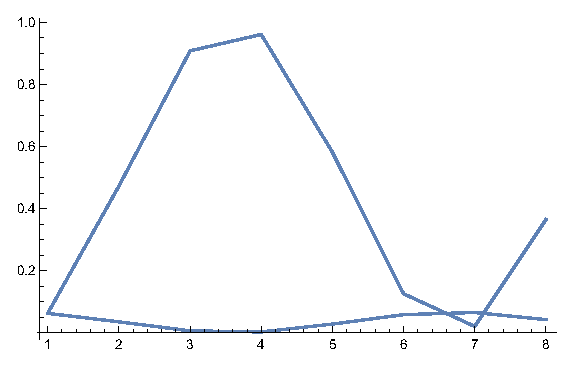
\includegraphics{Grover-2_gr1.eps}

\subsubsection*{Medir y probar resultado}

\begin{doublespace}
\noindent\(\pmb{\text{RandomChoice}\left[\text{Flatten}\left[\text{Abs}\left[\text{ket$\psi $}_n\right]{}^2\right]\to \text{Table}\left[i,\left\{i,1,\text{Dimensions}\left[\text{ket$\psi
$}_n\right][[1]]\right\}\right],20\right]}\\
\pmb{\text{Position}[\text{data},\text{buscar}]}\\
\pmb{\text{data}[[\text{Position}[\text{data},\text{buscar}][[1,1]]]]}\)
\end{doublespace}

\begin{doublespace}
\noindent\(\{1,1,1,1,1,1,1,14,1,1,1,1,1,1,1,1,1,1,1,1\}\)
\end{doublespace}

\begin{doublespace}
\noindent\(\{\{1\}\}\)
\end{doublespace}

\begin{doublespace}
\noindent\(16\)
\end{doublespace}

\end{document}
